\chapter{Introduction}

The inverted pendulum is a classical control system, aiming at getting a pendulum with its center of mass above the pivot point to balance, see \autoref{invertedPendulum}. The pendulum consists of a mass $m_p$ on a rod with length $l$, located on a moving base. A force $F_F$ is applied to the base, so the tilting angle of the pendulum, $\theta_p$, is minimized. 

Whereas a regular pendulum is a stable system with an equilibrium point, the inverted pendulum is inherently unstable. This means that unless some action is taken, the pendulum will fall over. To keep the pendulum balanced, it is necessary to measure the tilting angle $
\theta_p$, and, based on a model of the system, make the base move in the correct way by means of an applied force $F_F$.

%\begin{figure}[H]
%\centering
%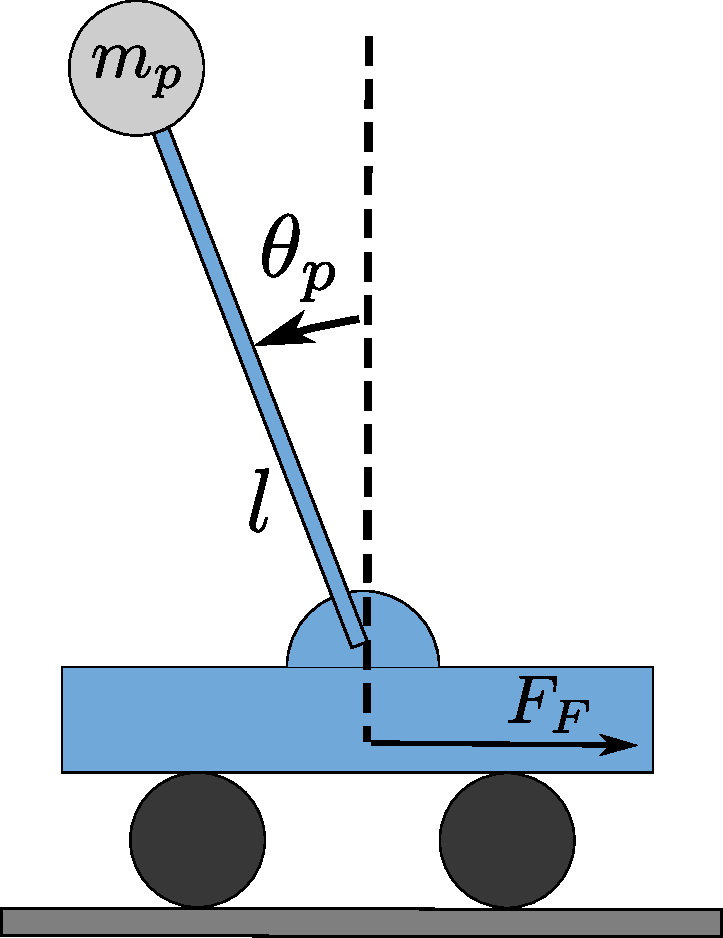
\includegraphics[width=0.4\textwidth]{figures/invertedPendulum.pdf}
%\caption{An inverted pendulum with mass \emph{m} placed on a moving base which is affected by a force $F$. The pendulum has length \emph{l}, and is currently tilted at an angle \emph{$\theta$}}
%\label{fig:invertedPendulum}
%\end{figure}

\begin{figure}[H]
\centering
	\begin{minipage}{0.45\textwidth}

	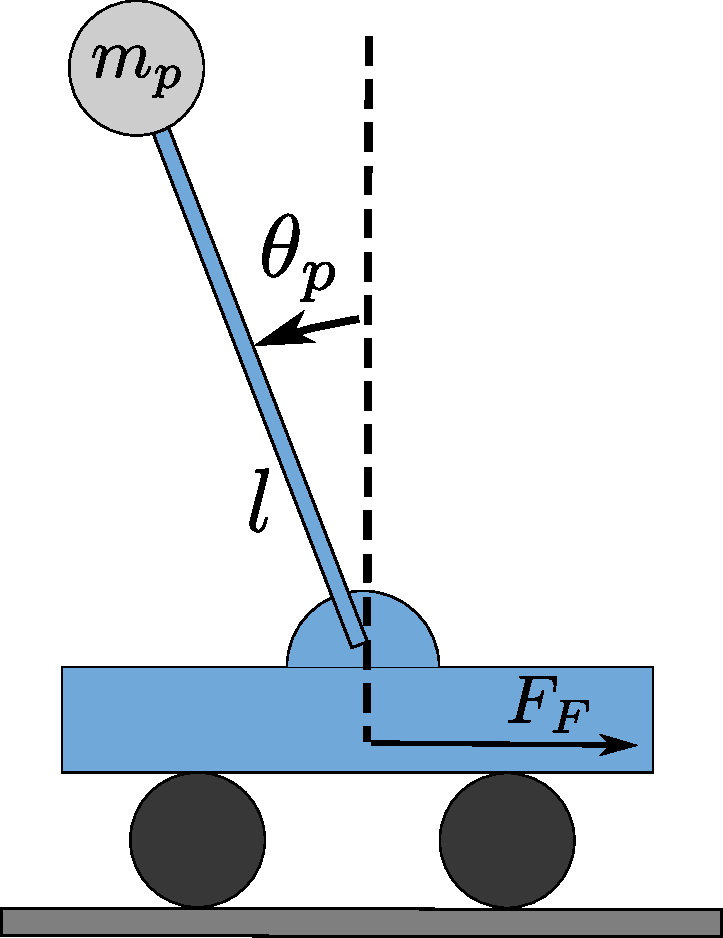
\includegraphics[width=0.9\textwidth]{figures/invertedPendulum.pdf}
	\caption{An inverted pendulum placed on a moving base}
	\label{invertedPendulum}
	\end{minipage}
	\hspace{0.08\textwidth}
	\begin{minipage}{0.40\textwidth}
	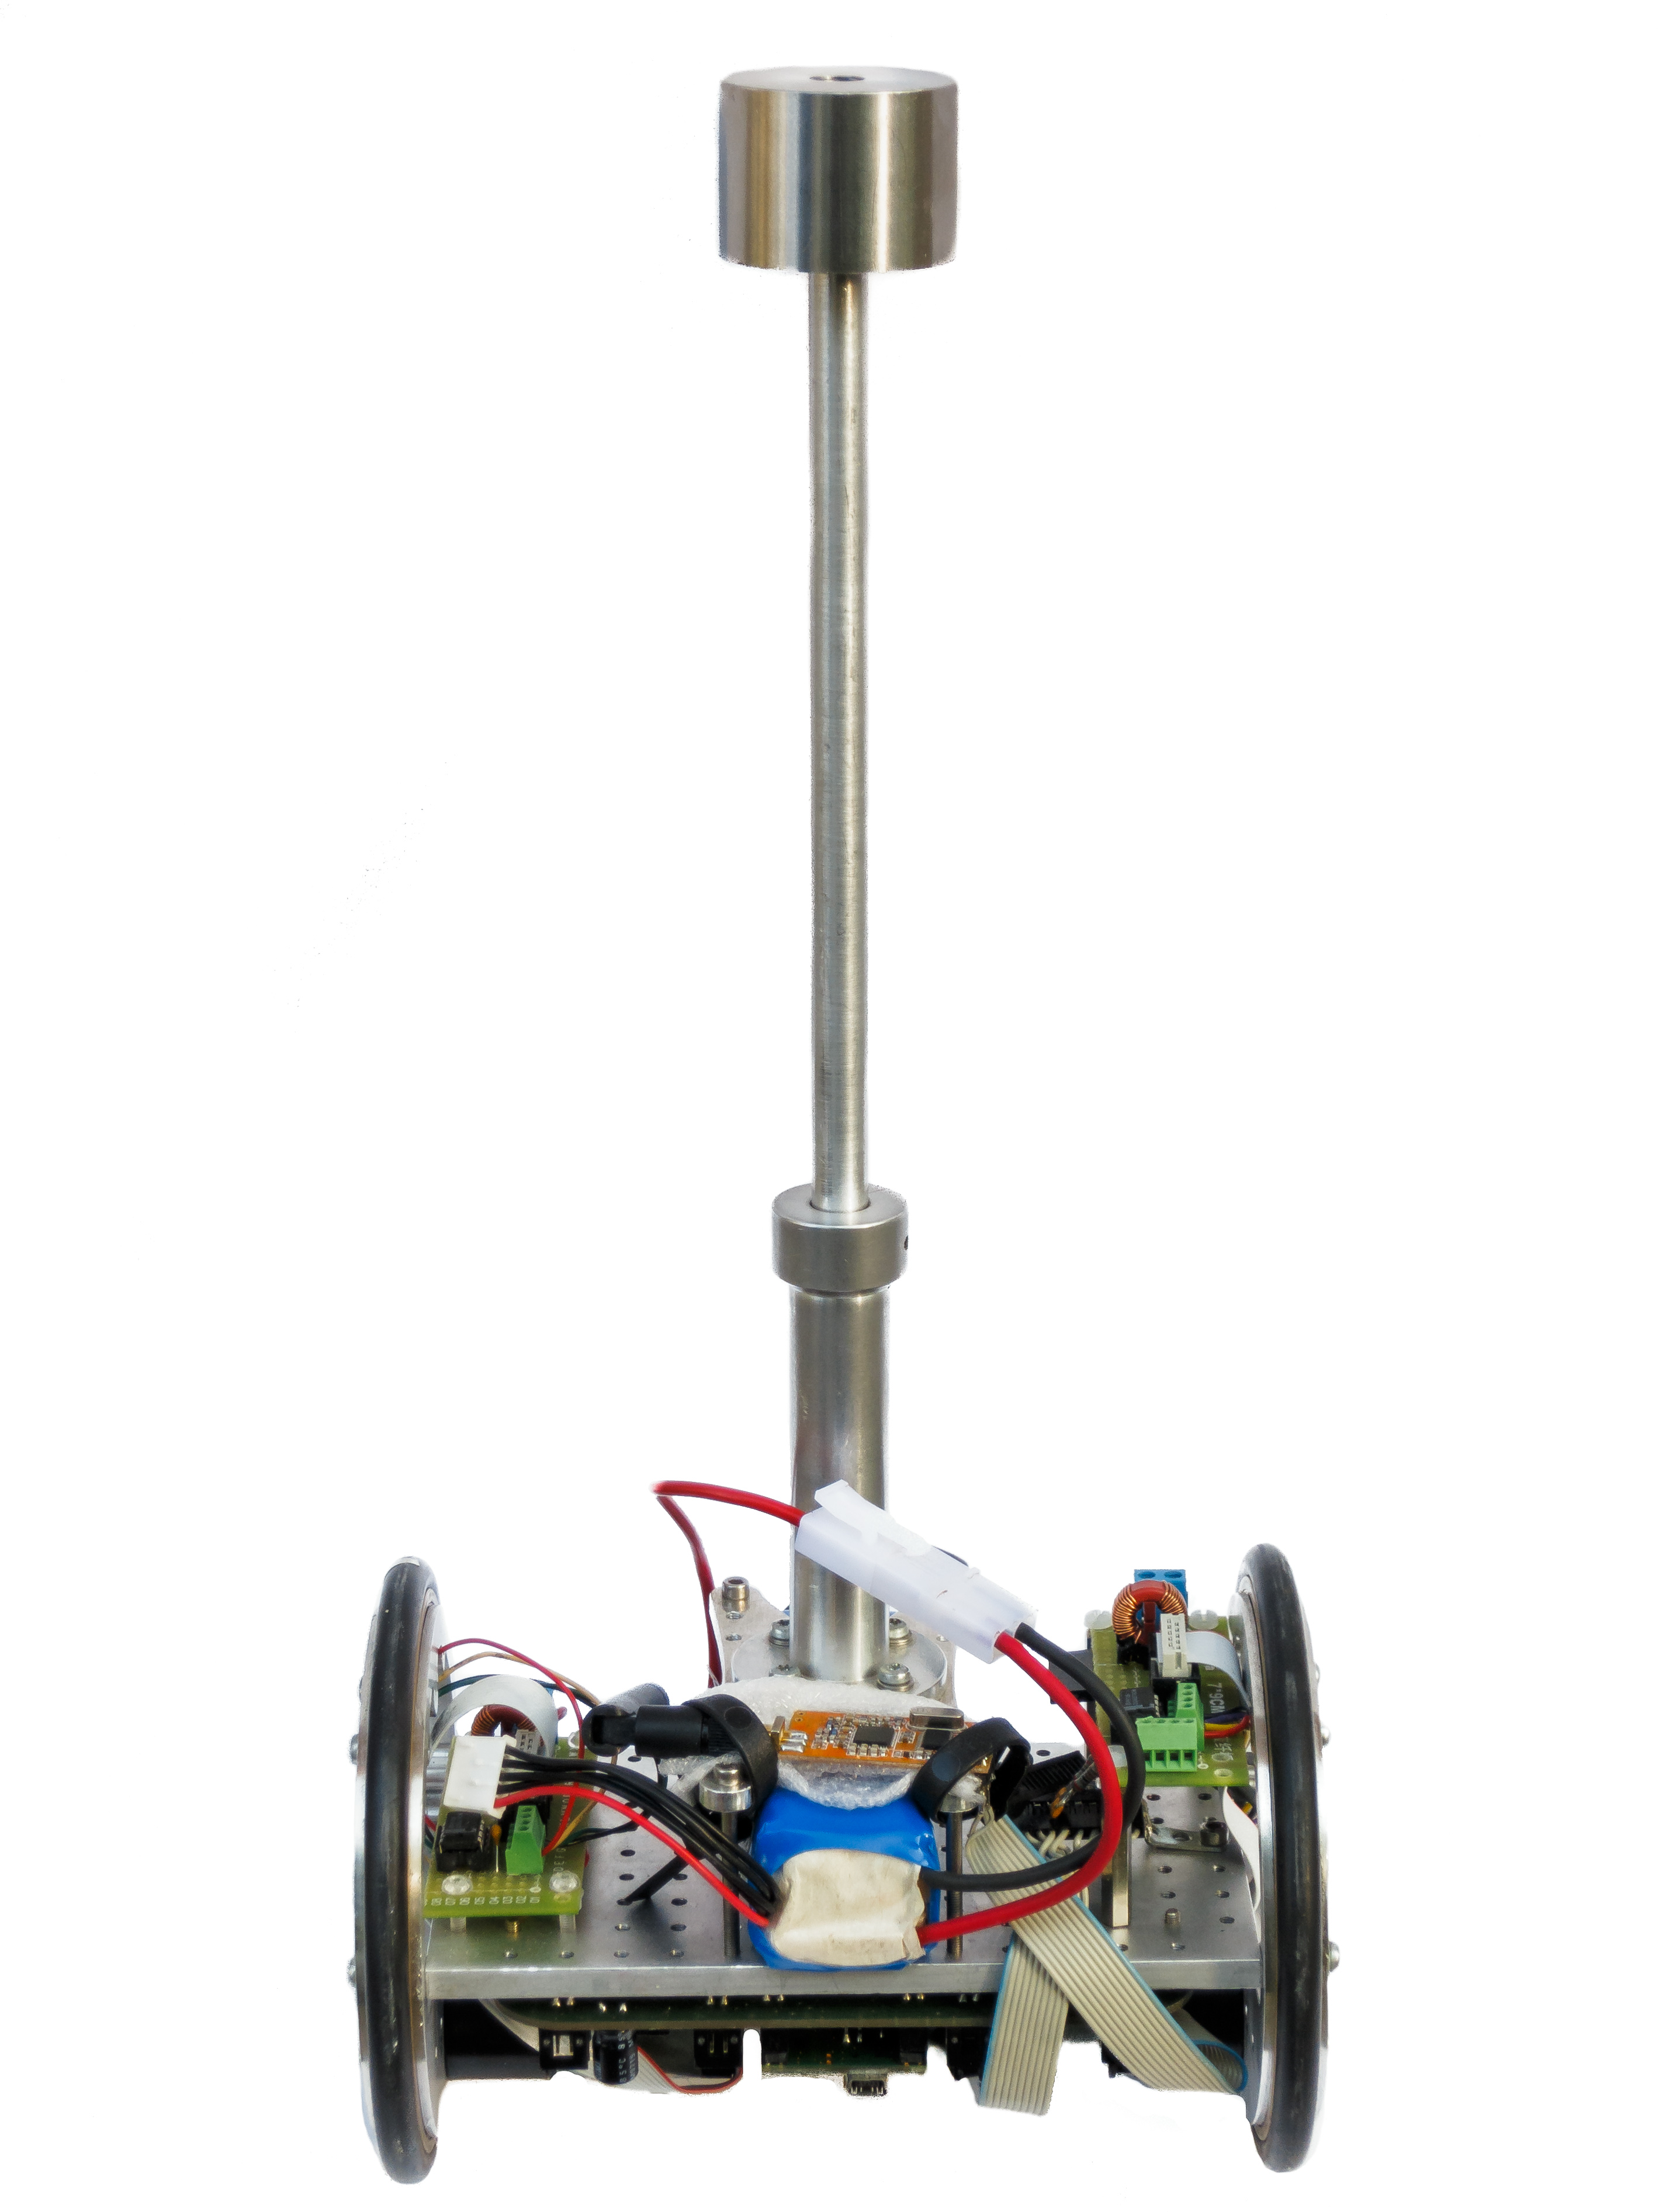
\includegraphics[width=\textwidth]{figures/hardwarePlatform.jpg}
	\caption{The segway to be used in the project (approx. height is 37 cm)}
	\label{minisegway}
	\end{minipage}
\end{figure}
%\todo{why is this interesting to work with}
\vspace{-3mm}
The inverted pendulum has found a new application in recent years, namely in the form of the segway. A segway is a small vehicle that can be used for human transportation where the user stands on a platform placed between two wheels.

%\begin{figure}[H]
%\centering
%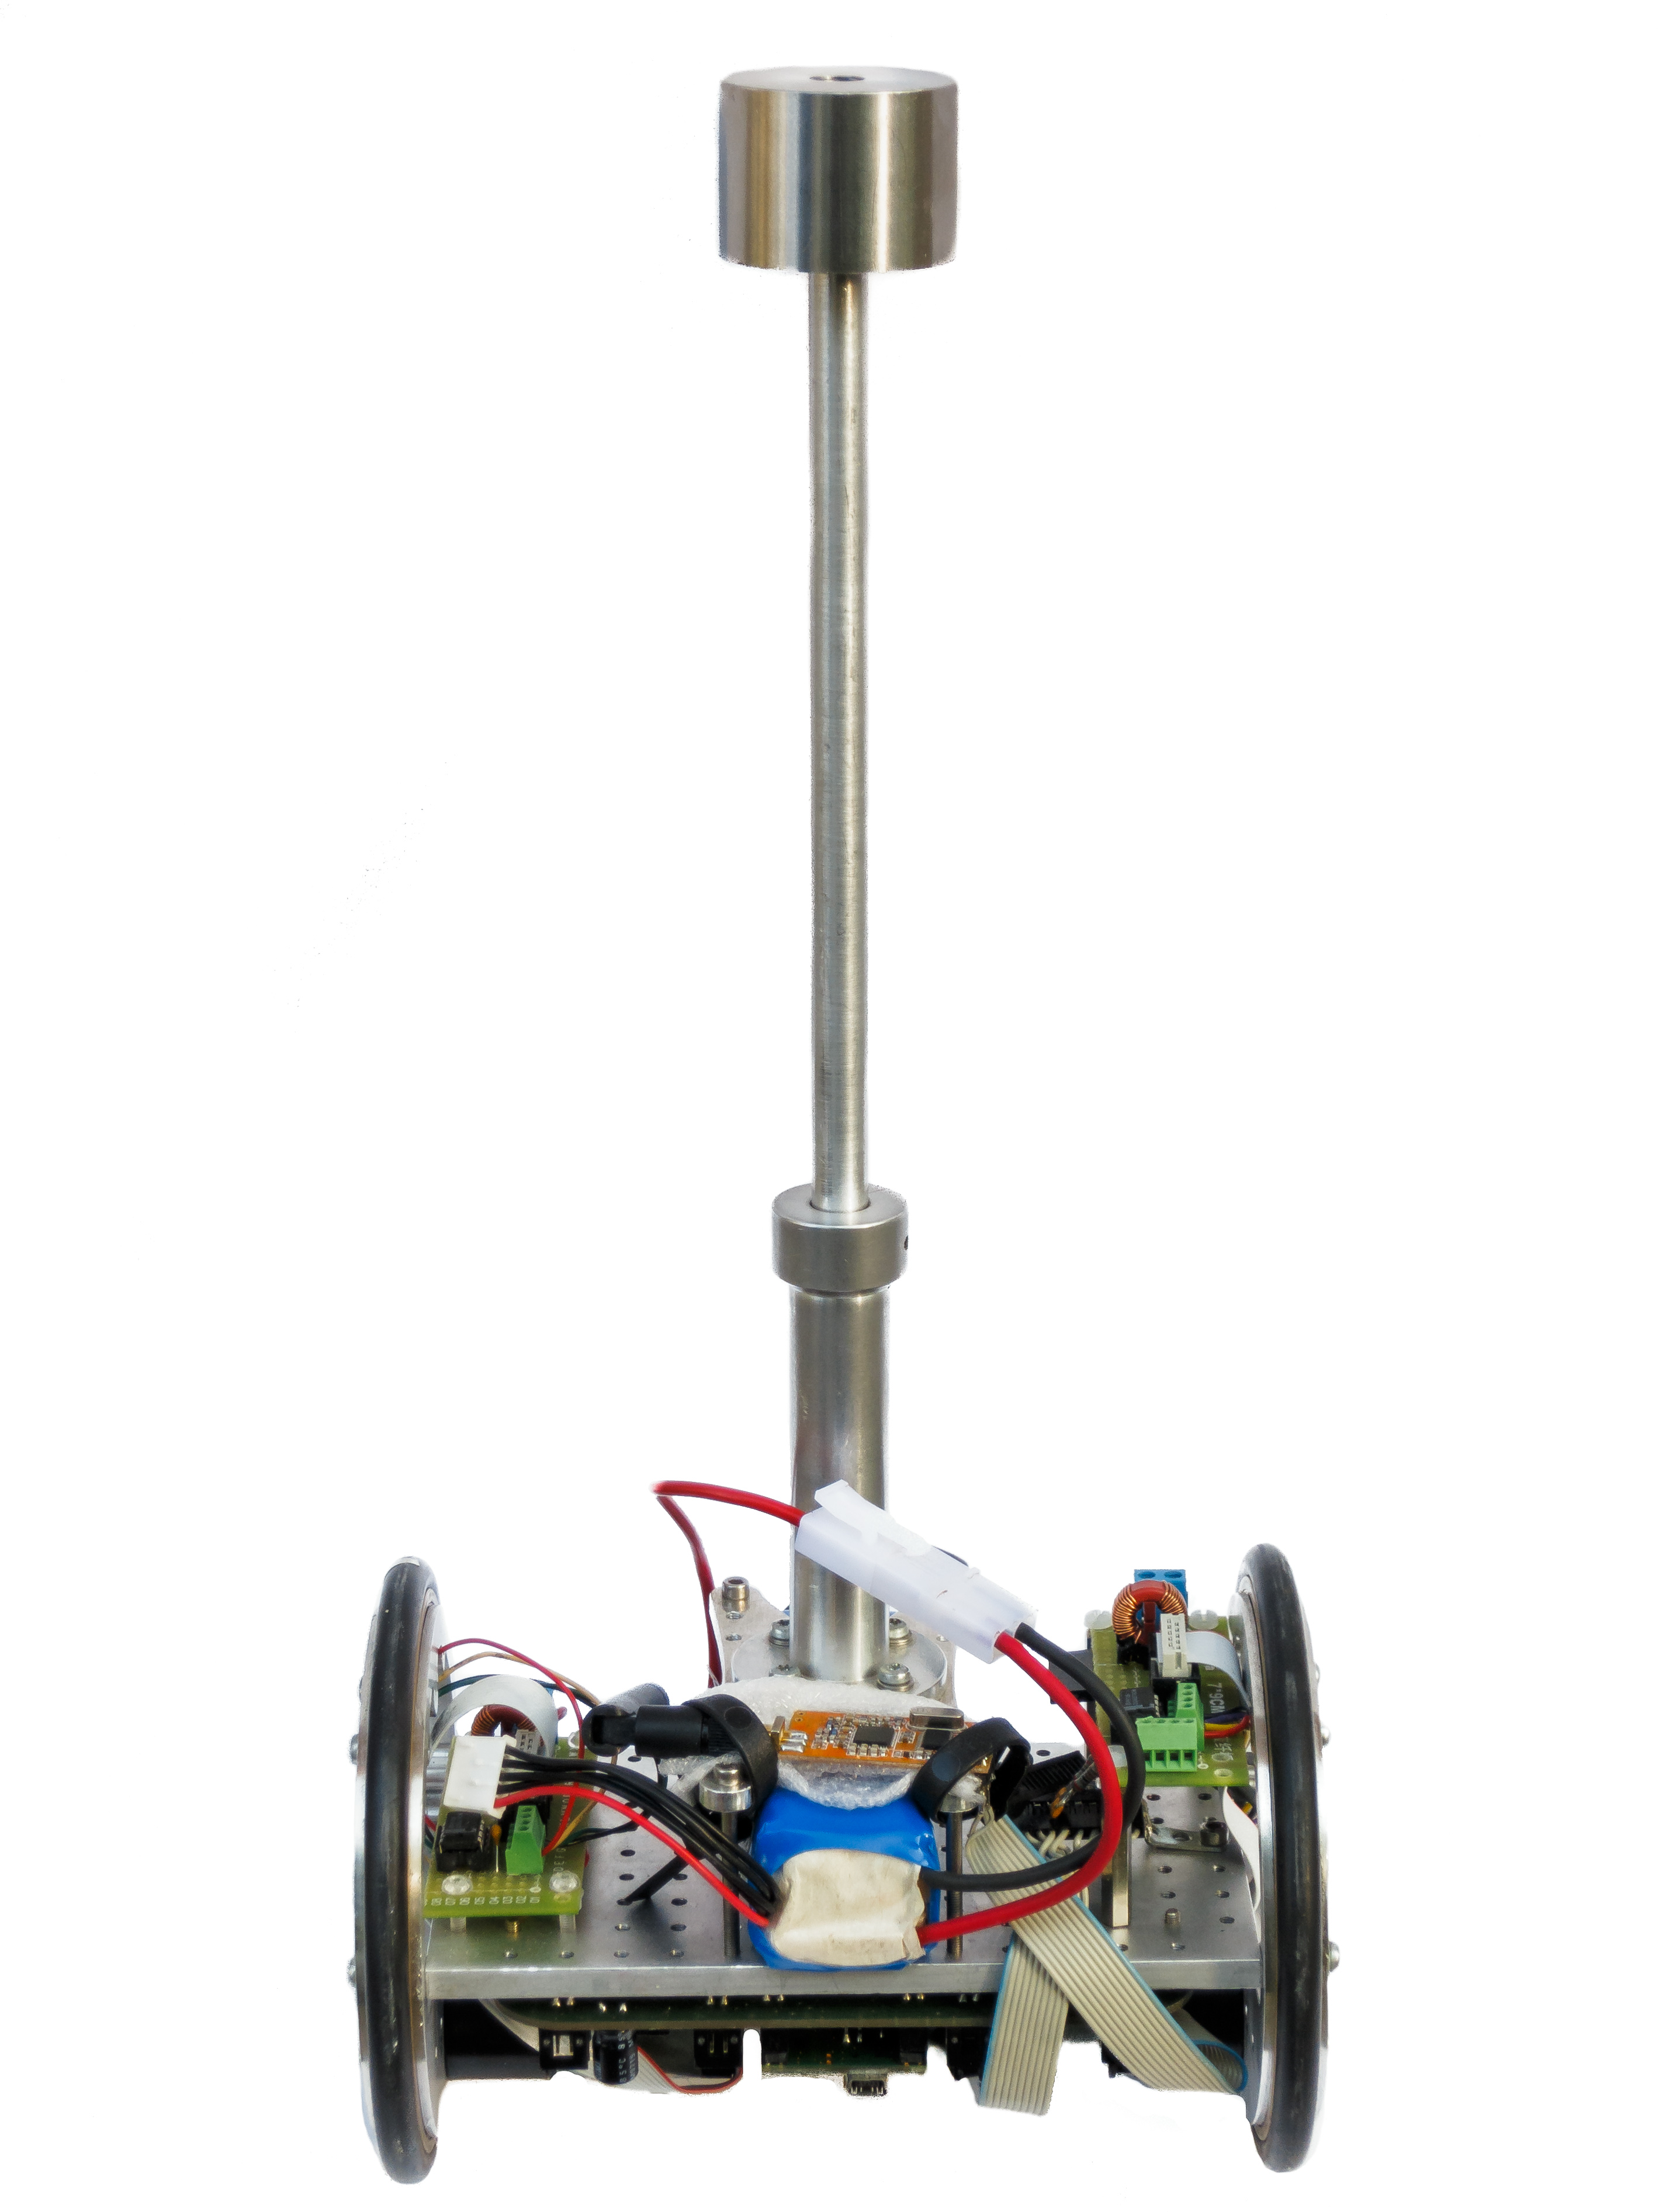
\includegraphics[width=0.4\textwidth]{figures/hardwarePlatform.jpg}
%\caption{The minisegway to be used in the project}
%\label{fig:minisegway}
%\end{figure}

This project concerns the development of a controller for a pre-manufactured segway provided by Aalborg University as can be seen in \autoref{minisegway}. This controller is to stabilize the inverted pendulum in it's upright position, and control the segway's position. The segway is seen as toy to be driven around indoors, and not as a model of a full-size segway. Because of this, all mentions and analyses of a segway throughout the report is in regards to the segway, and not a full-size segway.\\
In the following chapter, a presentation of the general workings of segway is presented.
%In order to control the balancing and driving of the segway, a controller has to be implemented. A good solution is to make the remote control wireless. %Therefore, a wireless remote for the segway will be discussed later on. \todo{a bit rough introduction to remote controller requirement}



%Before the actual modelling and controller design can take place, a presentation of this platform done in the following chapter.


%in particular the modelling and control needed to make the segway self-balancing.
%Ralf's suggestions:

%The inverted pendulum is a classical control problem, in which a pendulum, usually hanging beneath the pivot point, is inverted so that it hangs above.
%
%Whereas a regular pendulum is a stable system with a resting position, the inverted pendulum is inherently unstable. This means that unless some action is taken, the pendulum will fall over by itself. 
%
%The inverted pendulum has found a new application in recent years, namely in the form of the segway. A segway is a means for transportation, where the user stands on a platform placed on two wheels. The segway moves in the direction the user moves, i.e. if the user leans forward, the segway moves forward.
%
%This project concerns the development of a segway, in particular the modelling and control needed to make the segway self-balancing.
